\documentclass[11pt,spanish]{article} % Idioma
\usepackage{babel}
\usepackage[T1]{fontenc}
\usepackage{textcomp, verbatim} % \begin{comment}
\usepackage[utf8]{inputenc} % Permite acentos

\usepackage{wrapfig} % Imagenes %\graphicspath{ {./imagenes/} }
\usepackage[left=2.75cm,top=2.5cm,right=2cm,bottom=2.5cm]{geometry} % Márgenes
\usepackage{amssymb, amsmath, amscd, amsfonts, amsthm, mathrsfs } % Símbolos matemáticos
\usepackage{cancel} % Cancelar expresiones
\usepackage{multirow, multicol, tabularx, booktabs, longtable} % Tablas
\usepackage{fancyhdr, fncychap} % Encabezados
\usepackage{algpseudocode, algorithmicx, algorithm} % Pseudo-código
\usepackage{bbding} % Símbolos
\usepackage{enumitem} % Enumerados a), b), c)... usando \begin{enumerate}[label=\alph*)]
\usepackage{graphicx, xcolor, color, pstricks} % Gráficos --TikZ--
% http://www.texample.net/tikz/examples/
\usepackage[hidelinks]{hyperref}  % Enlaces
\usepackage{verbatim} % Comentarios largos \begin{comment}
\usepackage{rotating} % \begin{rotate}{30}
\usepackage[all]{xy} % Diagramas
\usepackage{xparse} % Entornos
\usepackage{listings}
\usepackage{biblatex} %Imports biblatex package
\addbibresource{bibliography.bib} %Import the bibliography file

\definecolor{codegreen}{rgb}{0,0.6,0}
\definecolor{codegray}{rgb}{0.5,0.5,0.5}
\definecolor{codepurple}{rgb}{0.58,0,0.82}
\definecolor{backcolour}{rgb}{0.95,0.95,0.92}

\lstdefinestyle{mystyle}{
	backgroundcolor=\color{backcolour},
	commentstyle=\color{codegreen},
	keywordstyle=\color{magenta},
	numberstyle=\tiny\color{codegray},
	stringstyle=\color{codepurple},
	basicstyle=\footnotesize,
	breakatwhitespace=false,
	breaklines=true,
	captionpos=b,
	keepspaces=true,
	numbers=left,
	numbersep=5pt,
	showspaces=false,
	showstringspaces=false,
	showtabs=false,
	tabsize=2
}
\lstset{style=mystyle}


% Comandos
\newcommand{\docdate}{}
\newcommand{\subject}{}
\newcommand{\docauthor}{Rubén Morales Pérez}
\newcommand{\docemail}{srmorales@correo.ugr.es}

\newcommand{\N}{\mathbb{N}}
\newcommand{\Q}{\mathbb{Q}}
\newcommand{\C}{\mathbb{C}}
\newcommand{\R}{\mathbb{R}}
\newcommand{\Z}{\mathbb{Z}}




\usepackage[final]{pdfpages}


\linespread{1.1}                  % Espacio entre líneas.
\setlength\parindent{0pt}         % Indentación para párrafo.

\title{  } % Required for table of contents
\author{ }
\date{ } % Required for table of contents



\begin{document}

\begin{center}
  
\includegraphics[scale=0.4]{img/logo_ugr.png}
\end{center}

\begin{center}
  \Large TRABAJO FIN DE GRADO\\ 
  \large Doble grado en Ingeniería Informática y Matemáticas
  \vspace{0.7cm}

  \hrule
  \vspace{0.2cm}
  \textbf{\LARGE MW Store: facilitador genérico para proveedores de servicios con multi-inquilinato en una infraestructura Cloud}
  \vspace{0.2cm}
  \hrule
  \vspace{2cm}
  
  \textbf{Autor}

  Rubén Morales Pérez

  \vspace{2cm}
  \textbf{Director}

  Manuel Isidoro Capel Tuñón

  \textit{Departamento de Lenguajes y Sistemas Informáticos}
\end{center}

\newpage

\ 
\thispagestyle{empty}

\maketitle
\tableofcontents % Generando el indice
\setlength\parindent{0pt} % Quitamos la sangría

\newpage

\section{Software infraestructure}

Example \cite{example}

\subsection{Functional overview}


\subsection{Architecture}
\subsubsection{Technological stack}
Front end: angular (testing with karma + jasmine)
Back end: java 17 (testing with junit)
Database: PostgreSQL
Continous integration and delivery: Jenkins
Orchestration: Docker + Kubernetes
End to end tests: Selenium

\subsubsection{Dependencies}

\subsection{Continuous integration and delivery}
\subsubsection{Deployments}
\subsubsection{Data migrations}


\subsection{Quality}
Feature development will be slower as the program grows. Development in youth programs is faster than development in mature programs due to code complexity and possible regressions.
Software must be carefully designed. Higher quality standards will prevent slowdowns in the development of new features, and regressions will be caught earlier (citation needed).


\subsubsection{Code quality}
SonarQube

\subsubsection{Automatic tests}
Automatic tests will catch bugs before production release.
There are several testing strategies that can be used together:
\begin{itemize}
	\item End to end tests: test entire workflows, involving front end, back end and database(s).
	\item Integration tests: specific use cases involving several components.
	\item Unit tests: test cases involving only one component, mocking other components when needed. In the back end, they don't involve the database, making them much faster.
\end{itemize}

The desired test amount proportion is described in the test pyramid:
\begin{figure}[H]
  \centering
  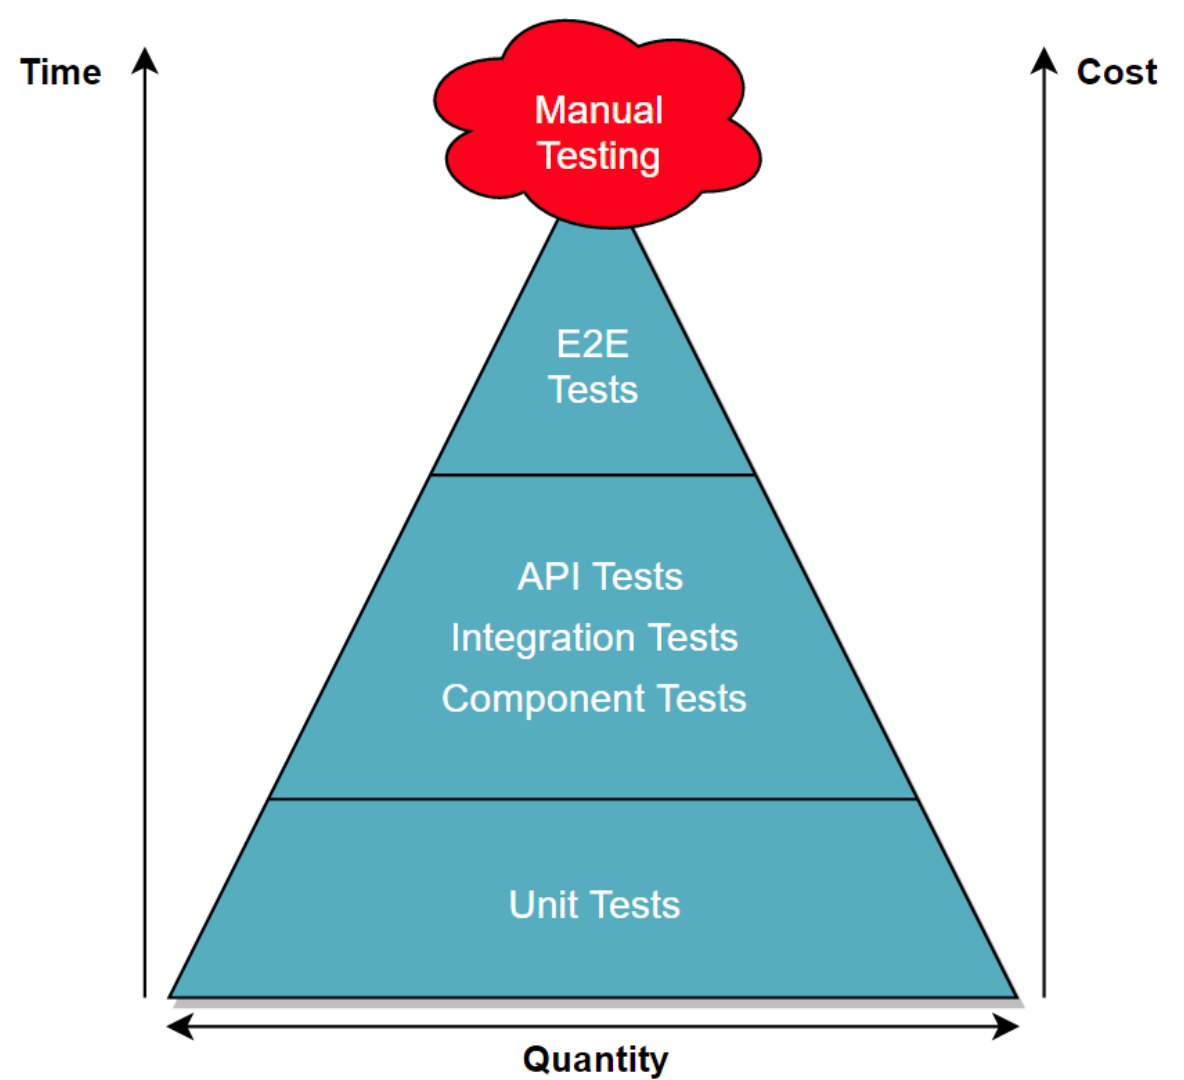
\includegraphics[scale=0.275]{img/test_pyramid.png}
  \caption{Test pyramid \cite{test-pyramid}}
\end{figure}

The inverted testing pyramid (fewer unit and integration tests, with an emphasis on automated and manual functional testing) is considered an anti-pattern, reducing the responsiveness, maintainability and reliability of the test setup \cite{test-pyramid}. 
Unit tests help identify faults in earlier phases \cite{test-pyramid} and must be the backbone of any software product.


\newpage
\section{Mathematical modelling}

\subsection{Petri nets}
\subsubsection{Reachability trees}

\subsection{Performance}
\subsubsection{Cache}

\subsection{Scalability}

\newpage


\printbibliography


\end{document}
